\documentclass{aip-cp}

\usepackage[numbers,sort&compress]{natbib}
\usepackage{rotating}
\usepackage{graphicx}
\usepackage[utf8]{inputenc}
\usepackage[russian]{babel}
\usepackage{xcolor}

%\makeatletter
%\def\@fnsymbol#1{\ensuremath{\ifcase#1\or *\or \dagger\or **\or
%   \ddagger\or \mathsection\or \mathparagraph\or \|\or \dagger\dagger
%   \or \ddagger\ddagger \or\mathsection\mathsection
%   \or \mathparagraph\mathparagraph \or *{*}*\or
%   \dagger{\dagger}\dagger \or\ddagger{\ddagger}\ddagger\or
%   \mathsection{\mathsection}\mathsection
%   \or \mathparagraph{\mathparagraph}\mathparagraph \else\@ctrerr\fi}}
%\makeatother

% Document starts
\begin{document}

% Title portion
\title{Shock-wave Thickness Influence to the Light Diffraction on a Plane Shock Wave}

\author[aff1,aff2]{Maksim Timokhin\corref{cor1}}
\author[aff1]{Mikhail Tikhinov}
\author[aff1]{Irina Mursenkova}
\author[aff1]{Irina Znamenskaya}

\affil[aff1]{Lomonosov Moscow State University, 119991, Moscow, Russia}
\affil[aff2]{Moscow Aviation Institute, 125993, Moscow, Russia}
\corresp[cor1]{Corresponding author: timokhin@physics.msu.ru}
%\authornote[note1]{This is an example of first authornote.}
%\authornote[note2]{This is an example of second authornote.}

\maketitle


\begin{abstract}

\end{abstract}

% Head 1
\section{INTRODUCTION}

Визуализация газовых течений. Теневые методы и проч. , книжки по теневым методам (добавить из тетрадки)

Дифракция света на ударной волне и ударноволновых конфигурациях

Ссылки на Сыщикову (добавить их), Panda \cite{Panda_1995} (+ ещй две)

Книжка и статья Hornig'a (добавить) - отражение света от фронта ударной волны

Сказать про электронный пучок как неоптический вариант визуализации (Muntz, Alsmeyer, Schmidt) 

Слова про цифровую обработку и проч. 

Структура плоской ударной волны 

эксперимент \cite{Schmidt_1969, Alsmeyer_1976, Pham-Van-Diep624}, 

аналитика \cite{Becker_1922, Mott-Smith_1951, Salwen_1964}, 

численные расчёты \cite{Kogan, Dodulad_Tcheremissine_2013, Rykov2008, ShockWaves_2015, Struchtrup_Torrilhon_2004, overshoot_2015} 

Optical methods of gas-dynamic flow visualization are based on a change in the optical path of light through inhomogeneities in the density of a transparent medium. Such optical methods include shadowgraph, schlieren, and interferometric methods \cite{}. Shadowgraph methods are most often used to visualize shock waves and to experimentally analyze shock-wave configurations \cite{}. At the same time, usually the aim of applying this approach is to fix the positions of the shock waves. 

In classical gas dynamics of inviscid gas shock waves are treated as discontinuities \citep{Sedov,LANDAU1987}. This fact implies that the average mean free path tends to zero in comparison with the flow scale. 

A rather simple method was proposed for numerically calculating the result of light diffraction by a plane shock of zero thickness in \cite{Pfeifer}. A jump in density leads to a jump in the refractive index of the medium and to a jump in the phase of the wave. A similar approach was used, for example, in \cite{Panda_1995} to calculate the light intensity after passing through a shock wave in front of a blunt body. The obtained numerical results of light intensity distribution on the screen are in excellent agreement with the presented experimental shadowgraph data \cite{Pfeifer,Panda_1995}.

It is well-known fact that for sufficiently dilute gases the shock-wave thickness constitutes several mean free paths (see e.g. \cite{Kogan, Cercignani_book}). Here we would like to investigate the shock thickness influence on the light diffraction results. The shock-wave structure problem has been studied analytically with different mathematical approaches \cite{Becker_1922, Mott-Smith_1951, Salwen_1964, Holway_1964, Yen_1966}. The structure of a plane shock wave has been investigated experimentally with optical and electron methods fluorescence methods \cite{Hornig_1950, Hansen_Hornig_1960, Robben, Alsmeyer_1976, Pham-Van-Diep624}. A lot of investigations were provided with kinetic approach. The numerical results of this approach, as well as the experimental data, became the reference for this flow. This way includes the numerical solution of Boltzmann kinetic equation  \citep{Ohwada_shock, Dodulad_Tcheremissine_2013, ShockWaves_2015}, model kinetic equations \citep{Shakhov, Rykov2008} and Direct Simulation Monte Carlo (DSMC) method \citep{Belotserkovskii, Pham-Van-Diep624, Erofeev_Friedlander_overshoot_2002, overshoot_2015}.

\section{PROBLEM FORMULATION AND MATHEMATICAL MODEL}

The values of the amplitude and phase are first determined at equidistant points immediately after the passage of the diffraction object. These points, by virtue of the Huygens-Fresnel principle, will be sources of secondary waves, the result of which is summed up at each observation point in accordance with their optical paths. Due to the one-dimensionality of the shock wave, cylindrical waves are used instead of spherical ones.

\begin{figure}
    \centerline{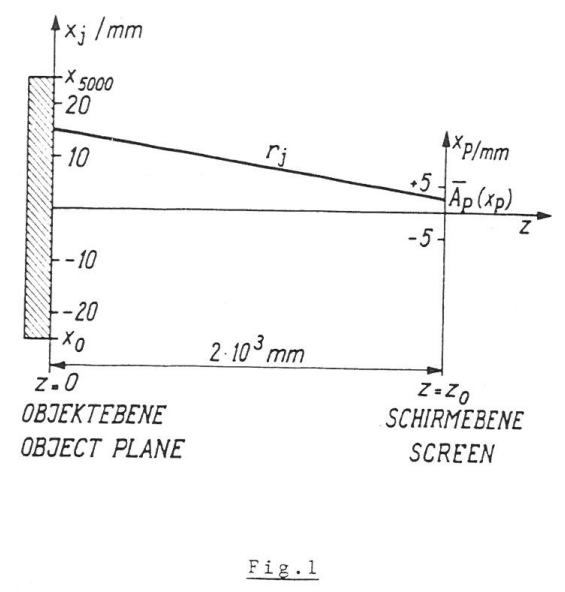
\includegraphics[width=160pt]{figures/fig1.png}}
\caption{ПЕРЕДЕЛАТЬ}
\label{fig1}
\end{figure}

In the plane of the object $z=0$, according to the Fig. \ref{fig1}, the density of the source points is more than 100 points per millimeter. Thus, with the assumed incident width, 50 mm plane wavefront, and distance $z_0 = 2$ m, more than two reference points are taken into account even in the outermost Fresnel zone. The complex amplitude $\overline{A}_p$ at the point $P{(x_p, z_0)}$ on the screen at the distance of $z_0$ from the plane of the object is calculated by the formula:
\begin{equation}
\overline{A}_p = \sum_{j=1}^{n} A_j \left(\frac{z_0}{r_j} \right)^{1/2} \exp \left(i \frac{2\pi}{\lambda} \left(r_j - z_0\right) + \Phi_j\right)
\end{equation}

where $n$ is the number of source points, $A_j$ is the magnitude of the amplitude at the $j$-th point, $\Phi_j$ is the initial phase at the $j$-th point and $\lambda$ is the light wavelength. $r_j$ is  defined as: $r_j = \left(z_0^2 + \left(x_j - x_P\right)^2\right)^{1/2}$. $x_j$ is the current coordinate at the plane near the diffraction object.

Написать про $Cos^2$ Fig. \ref{fig3}

As a validation of the numerical implementation the method, initially the test and experimental results from \cite{Pfeifer} were exactly reproduced.


Далее получение профиля плотности --> определение показателя преломления --> определение разности фаз для задания начальных данных

\begin{figure}
    \centerline{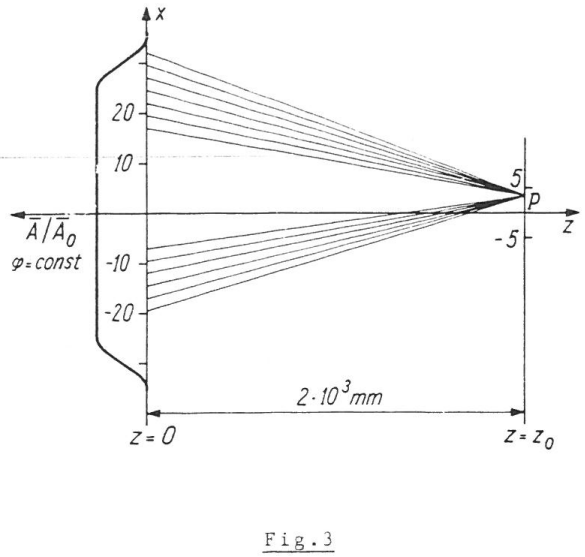
\includegraphics[width=160pt]{figures/fig3.png}}
\caption{ПЕРЕДЕЛАТЬ}
\label{fig3}
\end{figure}

\subsection{EXPERIMENTAL SETUP}

Описание из диссертации Орлова 2010 года

\section{RESULTS}

\subsection{Experimental case}

In Fig. \ref{Experiment_Ma2p1} a presents a shadow photograph obtained using the experimental setup described above. The shock wave moves from left to right. The pressure and temperature in front of the shock wave on the right are $p_0=25$ Torr and $T_0=293$ K, respectively. The Mach number of the shock wave is $Ma=2.1$. Fig. \ref{Experiment_Ma2p1} b shows the distribution of light intensity in an experiment obtained from \ ref {}.

\begin{figure}
\begin{tabular}{cc}
    {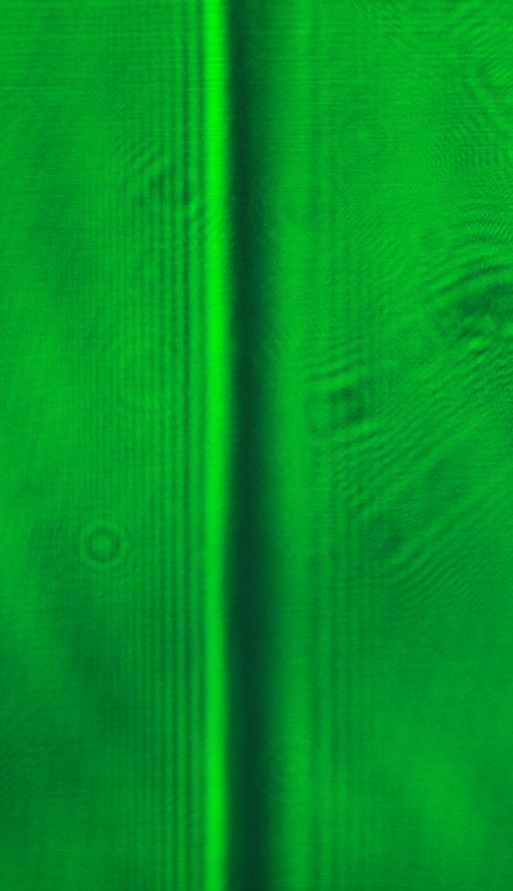
\includegraphics[width=185pt]{figures/Experiment_Ma2p1.jpg}}
    &{\includegraphics[width=185pt]{ numerical method}}\\ a&b
\end{tabular}
\caption{The shadowgraph image for $Ma=2.1$, $p_0=25$ Torr and $T_0=293$ K (a) intensity distribution.}
\label{Experiment_Ma2p1}
\end{figure}

Сравнение с экспериментальной картинкой 

\subsection{The dependence on shock thickness}

Несколько картинок при одном и том же значении числа Маха (?). Лучше для двух (слабая и сильная ударные волны). Одна экспериментальная с $Ma=2.1$ и какой-нибудь $Ma=8.0$.

Итоговые графики, иллюстрирующие зависимость от длины свободного пробега --> толщины.

\section{CONCLUSION}

% Acknowledgement
\section{ACKNOWLEDGMENTS}
The work carried out at Moscow State University was supported by the Russian Science Foundation (Grant No. ).

% References

\nocite{*}
\bibliographystyle{aipnum-cp}%
\bibliography{sample}%


\end{document}